\title{Homework 4 Report}
\author{
        Hooley Cheng \\
                Department of Mathematics\\
        University of Washington\\
        Seattle, WA, 98105, U.S.
           
}
\date{\today}

\documentclass[12pt]{article}


\usepackage{amsmath}
\usepackage{graphicx}
\usepackage{float}
\usepackage{listings}

\usepackage{titlesec}
\begin{document}
\maketitle

\begin{abstract}
In this project, we are going to use LDA to help us classify music bands and genre.
\end{abstract}

\section{Introduction and Overview}\
In this assignment, we first use sampling techniques to help use generate data from limited songs, and then split these data into train set and test set. After thatn, we apply our knowledge of LDA to them, and, hopefully, it might help us to classify them.
\section{Theoretical Background}
\subsection{Singular Value Decomposition}
SVD de-composites a Matrix $A$ in to three components $U, S, V$. and
\[A = USV\]
where $U$  is an $ m\times m$ real or complex unitary matrix, $S$ is an $ m\times n$ rectangular diagonal matrix with non-negative real numbers on the diagonal, and$V$ is a $ n\times n$ real or complex unitary matrix.
One of properties of $S$ is that if there are redundancy in our data, then there will only have several large numbers, with the rest of the singular values being very close to 0.
\subsection{Linear Discrimination Analysis}
The figure below gives a cartoon of the key idea involved in the LDA. IN our example, two data sets are considered and projected onto new bases. In the left figure, the projection shows the data to be completely mixed, not allowing for any reasonable way to separate the data from each other. In the right figure, which is the ideal caricature for LDA. The data are well separated with the means $\mu_1$ and $\mu_2$ being well apart when projected onto the chosen subspace. Thus the goal of LDA is two-fold: find a suitable projection that maximizes the distance between the inter-class data while minimizing the intra-class data.
For a two-class LDA, the mathematical formulation will be:
	\[w = argmax_x \frac{w^TS_bw}{w^TS_ww}\]
	
\begin{figure}[H]
\begin{tabular}{cc}
  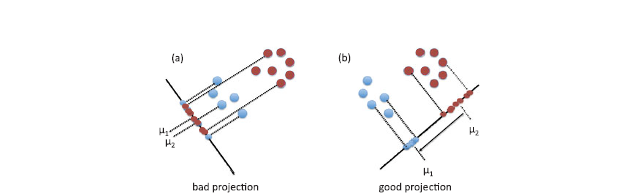
\includegraphics[width=\textwidth]{lda.png}
\end{tabular}
\end{figure}
\section{Algorithm Implementation and Development}
\subsection{Preparing Data}
First of all, we need to gather enough musical data for our tests. In order to do so, we downloads 27 songs from 3 different producers and 3 different genres. Then, we sampling 10 pieces of 5 second clips from each song to generate 270 clips in total for our tests.
\subsection{DLA Algorithm}
We first use SVD on our music data, and choose a limited number of the principal components as features. Once the SVD decomposition has been performed , the LDA is applied. We then use get our LDA projection basis as well as the decision threshold level associated with two different bands.
\subsection{Calculating Correctness}
In order to be aware of the performance of our algorithm, we need to apply our LDA projection basis on our test set to see how well the program has done its job.
\section{Computational Results}
\subsection{Band Classification}
The figure below shows that how well our algorithm works on training data of two different band sets.
\begin{figure}[H]
\begin{tabular}{cc}
  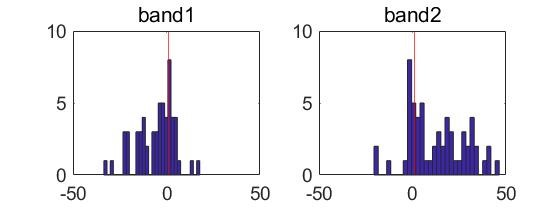
\includegraphics[width=\textwidth]{2band.jpg}
\end{tabular}
\end{figure}
Then we apply this algorithm to our test set:
\begin{figure}[H]
\begin{tabular}{cc}
  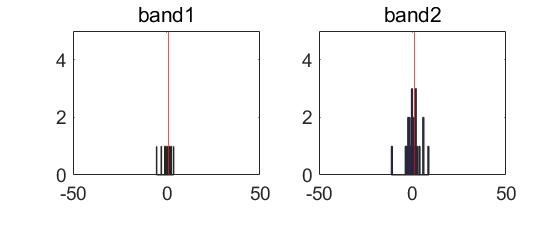
\includegraphics[width=\textwidth]{2band_test.jpg}
\end{tabular}
\end{figure}
However, we can see from the figure above do not classify test data well. Indeed, we checked our correctness rate and it is only 44\%, which is no better than flipping a coin. This result might due to the fact that we were over-fitting our data.
\subsection{Band Classification Within Same Genre}
In this section, we try our algorithm on different bands with same genre:
\begin{figure}[H]
\begin{tabular}{cc}
  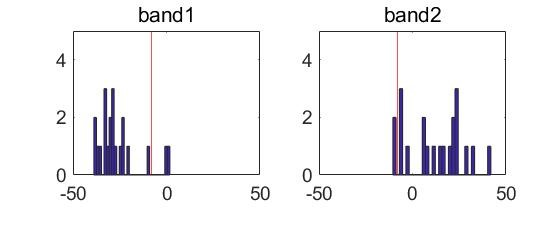
\includegraphics[width=\textwidth]{band_genre.jpg}
\end{tabular}
\end{figure}
Again, it performs almost perfect on trainning set, but very poor on test set. The successful rate is only 50\%
\begin{figure}[H]
\begin{tabular}{cc}
  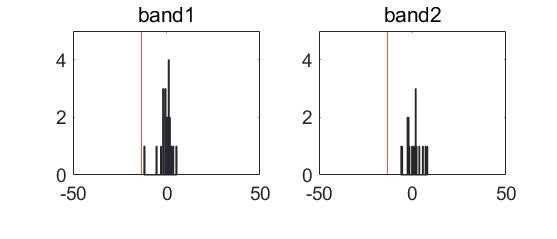
\includegraphics[width=\textwidth]{2band_genre_test.jpg}
\end{tabular}
\end{figure}
\subsection{Genre Classification}
Then, we train our algorithm on different genres.
\begin{figure}[H]
\begin{tabular}{cc}
  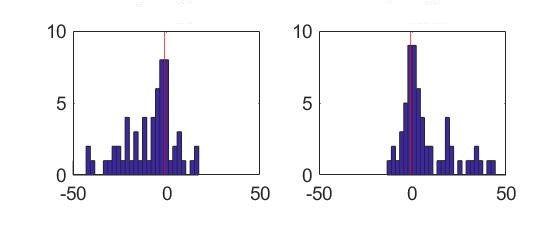
\includegraphics[width=\textwidth]{genre.jpg}
\end{tabular}
\end{figure}
Here, we also tried it on test set, it works bad still.
\begin{figure}[H]
\begin{tabular}{cc}
  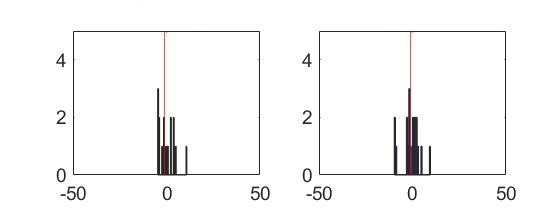
\includegraphics[width=\textwidth]{genre_test.jpg}
\end{tabular}
\end{figure}
\section{Summary and Conclusions}
We implement our DLA Algorithm and it performs well only on training set. This might due to the fact that sampling pieces over one single song could lead to over-fitting. So, preparing data become a very important part of Machine Learning, and "big data" is vital for the correctness for any algorithms.
\section{Appendix A}
SVD de-composites a Matrix $A$ in to three components $U, S, V$. and
\[A = USV\]
where $U$  is an $ m\times m$ real or complex unitary matrix, $S$ is an $ m\times n$ rectangular diagonal matrix with non-negative real numbers on the diagonal, and$V$ is a $ n\times n$ real or complex unitary matrix.
One of properties of $S$ is that if there are redundancy in our data, then there will only have several large numbers, with the rest of the singular values being very close to 0.
\section{Appendix B: Matlab Source Code}
\section{MATLAB codes}
\begin{verbatim}
Fs = 44100;
sample_num = 10;
duration = 5;

files_struct = dir('*.mp3');
files_table = struct2table(files_struct);
songs = string(files_table.name);
num = length(songs);
data = zeros(num * sample_num, Fs * duration);
y = zeros(num * sample_num, 2); 


for i = 1:num
    [v,] = audioread(songs(i));
    v = v(10*Fs:length(v) - 10*Fs - 1, 1);
    r = ceil(rand(1, sample_num) .* (length(v) - duration * Fs));
    hiphop = contains(songs(i),'Hiphop');
    rb = contains(songs(i), 'RB');
    jazz = contains(songs(i), 'Jazz');
    otis = contains(songs(i), 'Otis');
    maxwell = contains(songs(i), 'Maxwell');
    quincas = contains(songs(i), 'Quincas');
    if otis == 1
        y((i - 1) * sample_num + 1:i * sample_num, 1) = 1;
    elseif maxwell == 1
        y((i - 1) * sample_num + 1:i * sample_num, 1) = 2;
    elseif quincas == 1
        y((i - 1) * sample_num + 1:i * sample_num, 1) = 3;
    end
    
    if hiphop == 1
        y((i - 1) * sample_num + 1:i * sample_num, 2) = 1;
    elseif rb == 1
        y((i - 1) * sample_num + 1:i * sample_num, 2) = 2;
    elseif jazz == 1
        y((i - 1) * sample_num + 1:i * sample_num, 2) = 3;
    end
    
    for j = 1 : 10
        head = r(1, j);
        data((i - 1) * sample_num + j, :) = v(head:head + Fs*duration - 1, 1);
    end
end


total_sample = length(data(:, 1));
r = randperm(total_sample);
train = data(r(1:total_sample * 0.7), :);
train_y = y(r(1:total_sample * 0.7), :);
test = data(r(total_sample * 0.7 + 1 : total_sample * 0.9), :);
test_y = y(r(total_sample * 0.7 + 1 : total_sample * 0.9), :);
vali = data(r(total_sample * 0.9 + 1:end), :);
vali_y = y(r(total_sample * 0.9 + 1:end), :);
\end{verbatim}

\begin{verbatim}


function [result,w,U,S,V,threshold] = band_trainer(band1_com,band2_com,feature)
l = length(band1_com(1,:));
[U,S,V] = svd([band1_com, band2_com], 'econ');
bands = S * V';


U = U(:,1:feature);
band1 = bands(1:feature, 1:l);
band2 = bands(1:feature, l+1:2*l);

mb1 = mean(band1,2);
mb2 = mean(band2,2);
Sw = 0;
for i=1:l
    Sw = Sw + (band1(:, i)-mb1) * (band1(:, i)-mb1)';
end
for i=1:l
    Sw = Sw + (band2(:, i)-mb2) * (band2(:, i)-mb2)';
end
Sb = (mb1 - mb2) * (mb1 - mb2)';
[V2, D] = eig(Sb, Sw);
[~, ind] = max(abs(diag(D)));
w = V2(:,ind);
w = w/norm(w,2);
vband1=w'*band1;
vband2=w'*band2;
result = [vband1,vband2];
if mean(vband1) > mean(vband2)
    w = -w;
    vband1 = -vband1;
    vband2 = -vband2;
end

sortband1 = sort(vband1);
sortband2 = sort(vband2);
t1 = length(sortband1);
t2 = 1;
while sortband1(t1) > sortband2(t2)
    t1 = t1 - 1;
    t2 = t2 + 1;
end
threshold = (sortband1(t1) + sortband2(t2)) / 2;
close all
figure(1)
subplot(2,2,1)
hist(sortband1,30); hold on, xline(threshold, 'r');
set(gca,'Xlim',[-50 50],'Ylim',[0 10],'Fontsize',[14])
title('band1')
subplot(2,2,2)
hist(sortband2,30,'r'); hold on, xline(threshold, 'r');

set(gca,'Xlim',[-50 50],'Ylim',[0 10],'Fontsize',[14])
title('band2')
end


\end{verbatim}
\begin{verbatim}
[result,w,U,S,V,threshold] = band_trainer(band1_com,band2_com,feature);



test1 = test(test_y(:,2) ~= 3, :)
test1_y = test_y(test_y(:,2) ~= 3, 2);
test_mat = U'*test1';
pval = w'*test_mat;
ResVec = (pval>threshold);

test1_1 = w'*(U'*test(test_y(:,2) == 1, :)');
test1_2 = w'*(U'*test(test_y(:,2) == 2, :)');
close all
figure(2)
subplot(2,2,1)
hist(test1_1,30); hold on, xline(threshold, 'r');
set(gca,'Xlim',[-50 50],'Ylim',[0 5],'Fontsize',[14])
title('band1')
subplot(2,2,2)
hist(test1_2,30,'r'); hold on, xline(threshold, 'r');

set(gca,'Xlim',[-50 50],'Ylim',[0 5],'Fontsize',[14])
title('band2')

corr = 0;
for i=1:length(test1(:,1))
    if (test1_y(i) == 1 && ResVec(i) == 0)
        corr = corr + 1;
    end
    
    if (test1_y(i) == 2 && ResVec(i) == 1)
        corr = corr + 1;
    end
    
end

corr / length(test1(:,1))

\end{verbatim}
\end{document}